%!TEX TS-program = xelatex
\documentclass[10pt,twoside,BCOR12mm,DIV11,headinclude=false,footinclude=false]{scrreprt}

%%

%\usepackage{makeidx}
%\makeindex

%%%%%%%%%%%%%%%%%%%%%%%%%%%%%%%%%%%%%%%
%
%    FONTS   % % % 
%
%%%%%%%%%%%%%%%%%%%%%%%%%%%%%%%%%%%%%%%

\usepackage{fontspec}


%%%

\setromanfont[Mapping=tex-text]{Cambria}
\setsansfont{Helvetica Neue Light}
\setmonofont[Scale=MatchLowercase]{Menlo}
\newfontfamily\devfont[Renderer=Graphite,Script=Devanagari,Language=Sanskrit]{Annapurna SIL}
\newfontfamily\tamfont[Script=Tamil,Language=Tamil]{Arial Unicode MS}

\newfontinstance\devbfont[Renderer=Graphite,Script=Devanagari,Language=Sanskrit]{Annapurna SIL Bold}

\newcommand{\scb}[1]{\textbf{\textsc{#1}}}
\newcommand{\infont}[1]{\textsc{\scriptsize #1}}
\newcommand{\embf}[1]{\textbf{\emph{#1}}}
\newcommand{\echov}[1]{\textrm{\scriptsize #1}}
%%%%%%%%%%%%%%%%%%%%%%%%%%%%%%%%%%%%%%%%
%
%    PAGE LAYOUT   % % %
%
%%%%%%%%%%%%%%%%%%%%%%%%%%%%%%%%%%%%%%%%

\typearea[current]{classic}
\usepackage[headsepline,automark]{scrpage2}

% * GENERAL PAGE LAYOUT SETTINGS * * * * * * * * * * * * * * * * * * * * * * 

\setkomafont{pagenumber}{\normalfont\sffamily\bfseries}

\newcommand{\myversion}{\begin{scriptsize}Lazarus Project (Cologne Sanskrit Lexicon) Project Documentation 2\end{scriptsize}}



% * * FXRU HEADINGS * * * * * * * * * * * * * * * * * * * * * * * * * * * * * * *

\newpagestyle{fxruheadings}{%
{\rightmark\hfill}%
{\hfill\rightmark}%
{\hfill}%
(\textwidth, .4pt)}%
{%
{\pagemark \quad \vline \quad  \textit{\leftmark} \hfill  \myversion}%
{ \myversion\hfill \textit{\leftmark} \quad \vline \quad \pagemark}%
{\hfill\pagemark \hfill}%
}

% * * FXRU LEX HEADINGS * * * * * * * * * * * * * * * * * * * * * * * * * * * * * * *

% TO DO


% * * FXRU APPENDIX HEADINGS * * * * * * * * * * * * * * * * * * * * * * * * * * * * * * *

\newpagestyle{fxrutextheadings}{%
{\rightmark\hfill}%
{\hfill\rightmark}%
{\hfill}%
(\textwidth, .4pt)}%
{%
{\pagemark \quad \vline \quad  \textit{\rightmark} \hfill  \myversion}%
{ \myversion\hfill \textit{\rightmark} \quad \vline \quad \pagemark}%
{\hfill\pagemark \hfill}%
}


%%

%\usepackage[headsepline,automark]{scrpage2}
%\pagestyle{scrheadings}
\pagestyle{fxruheadings}
\automark[chapter]{subsection}
\pagenumbering{arabic}



% LAYOUT STRUCTURE %%%%%%%%%%%%%%%%%%%%%%%%%%%%

\setcounter{secnumdepth}{5}
\setcounter{tocdepth}{5}

%%%%%%%%%%%%%%%%%%%%%%%%%%%%%%%%%%%%%%%%%
%%%%%%%%%%%%%%%%%%%%%%%%%%%%%%%%%%%%%%%%%

%  OTHER PACKAGES       %%%%%%%%%%%%%%%%%%%%%%%%%%%%

\usepackage{rotating}
\usepackage{multicol}
\usepackage{natbib}
\usepackage{graphicx}


%Test features%%%%%%%%%%%%%%%%%%%%%%%%%%%%%%
\usepackage{xltxtra}
\usepackage{hyperref}
\hypersetup{								%
unicode=true,								%
pdftex, 										%
colorlinks=true, 							% 
linkcolor=black,  						%
citecolor=black, 							%
filecolor=black,  							%
pagecolor=, 								%
urlcolor=black,  							%
pdftitle={Vedic Accent and Lexicography}, 	%
pdfauthor={Felix Rau} 				%
}

\def\partautorefname{part}
\def\chapterautorefname{\S}
\def\sectionautorefname{\S}
\def\subsectionautorefname{\S}
\def\subsubsectionautorefname{\S}
\def\paragraphautorefname{\S}

%%%%%%
\usepackage{gb4e}



\begin{document}

\subject{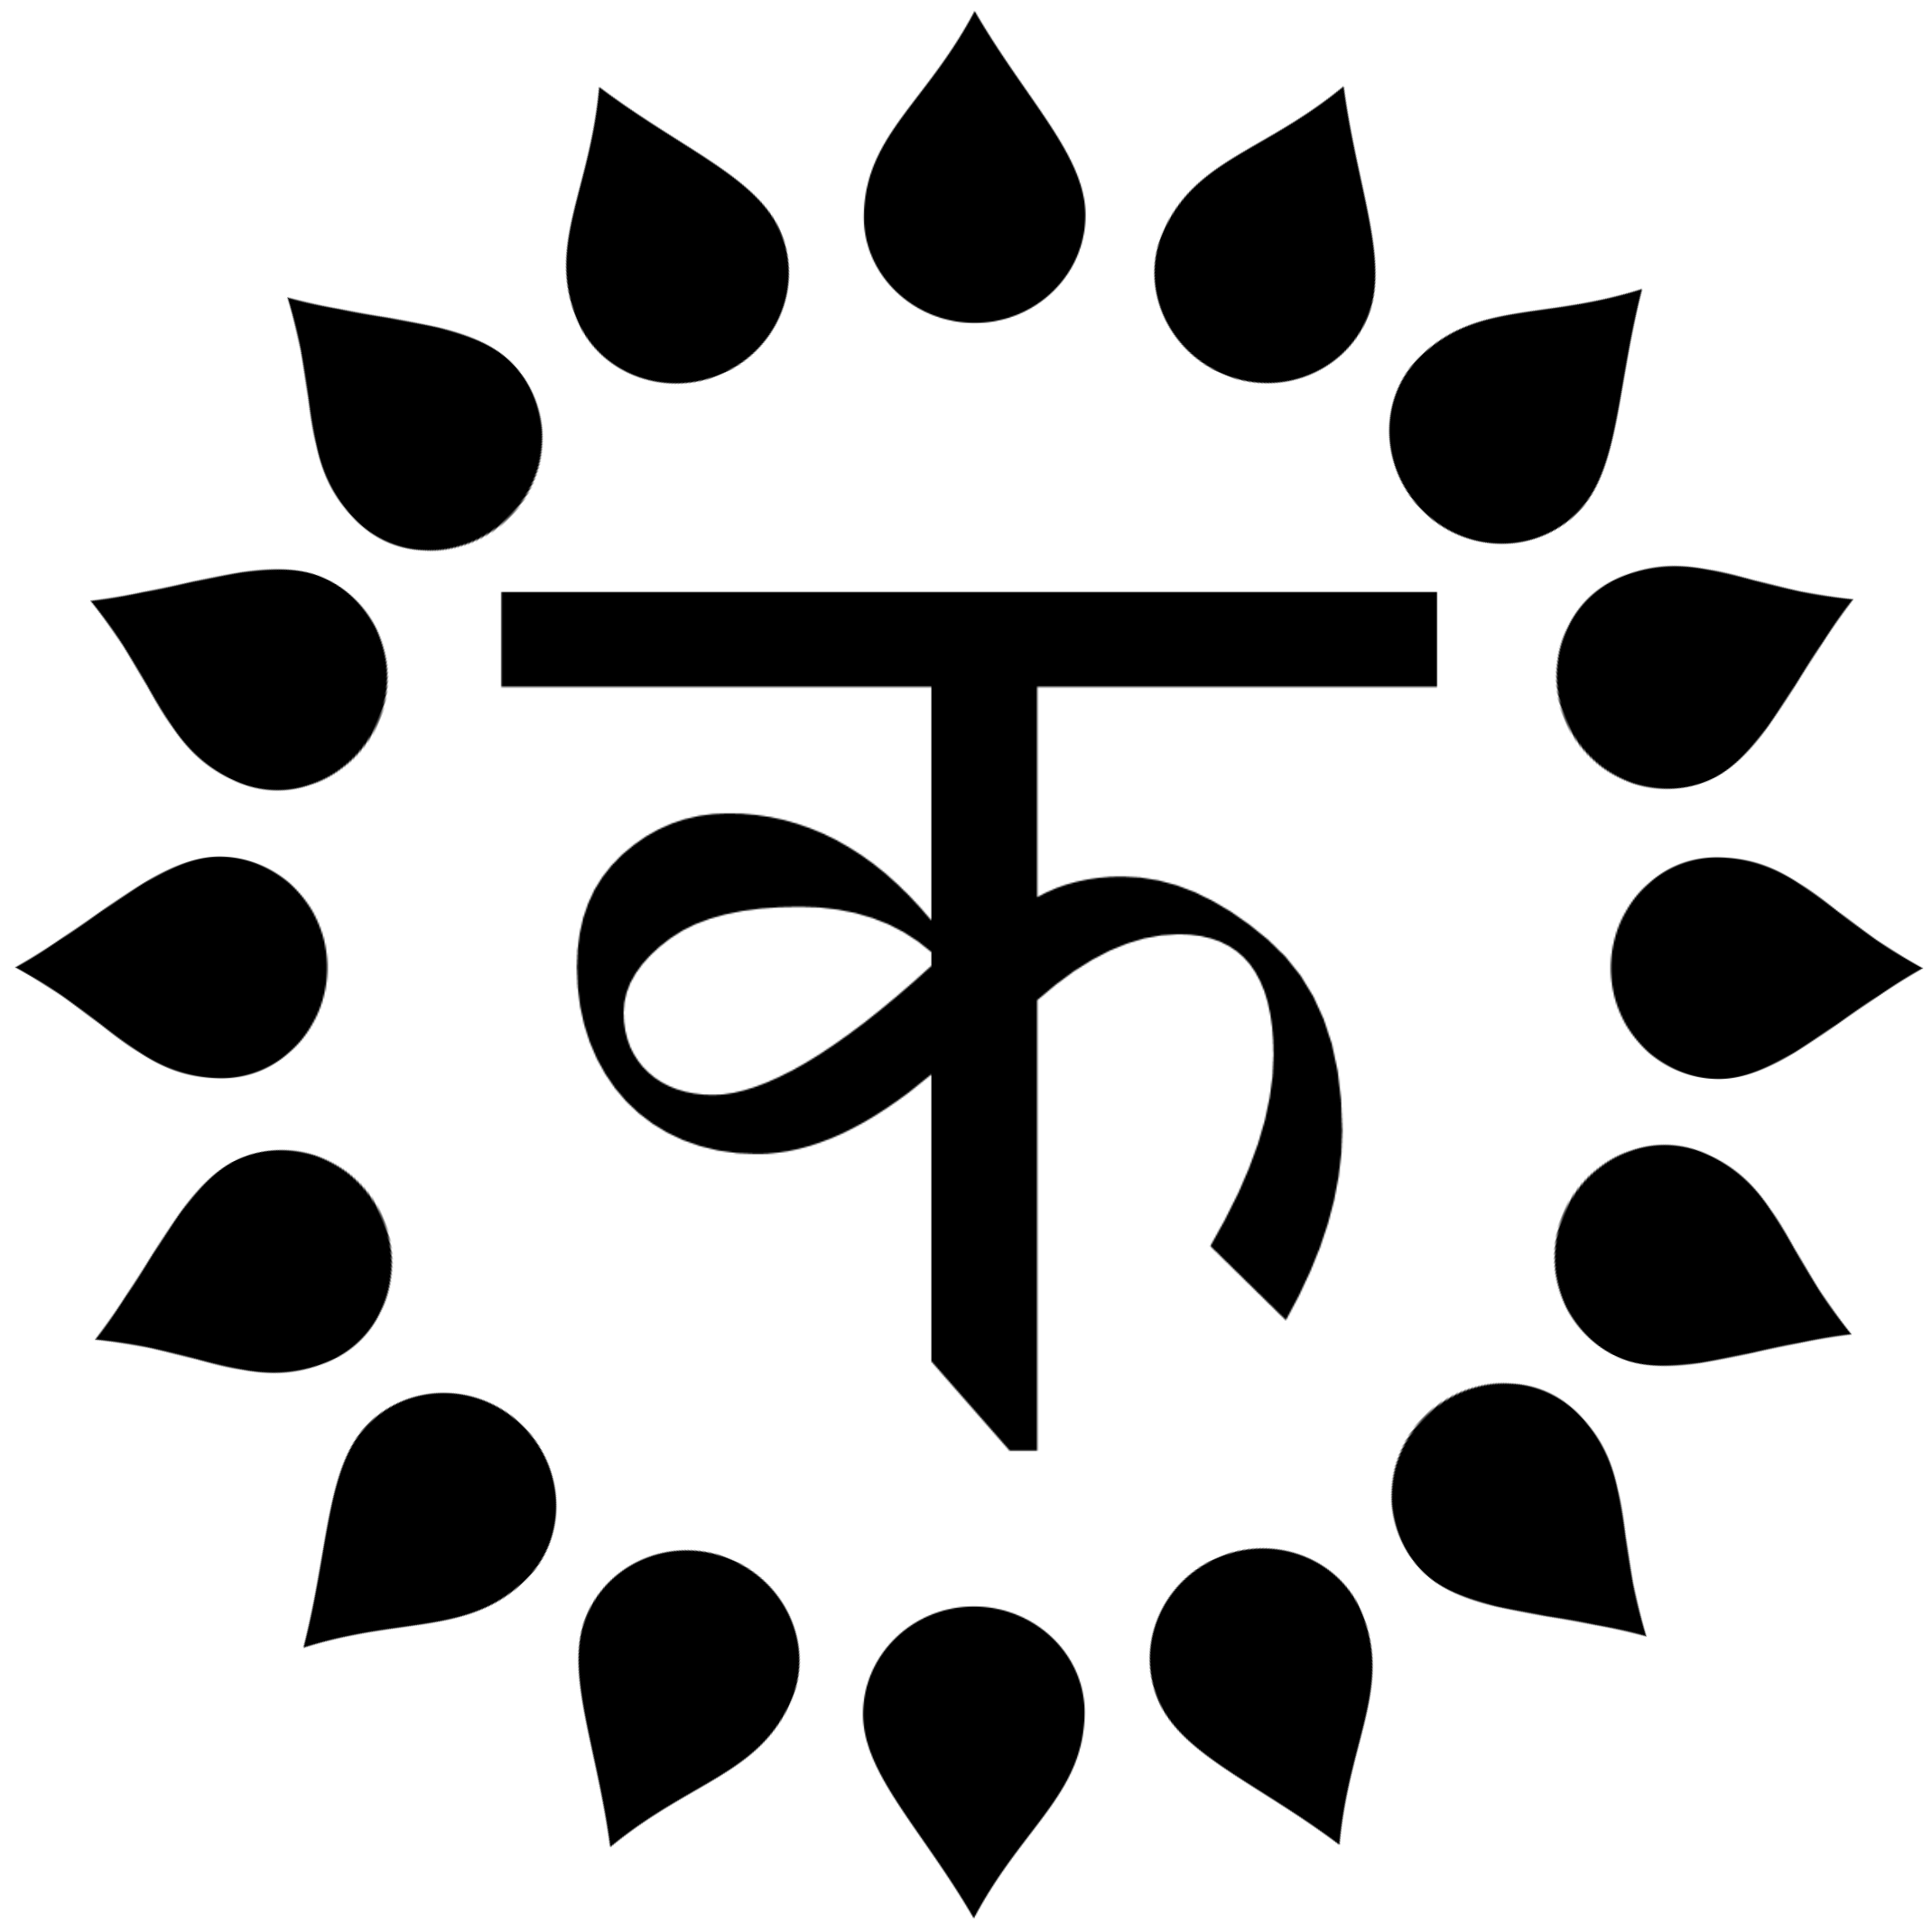
\includegraphics[width=4cm]{./imgs/cdsl-logo.png}}
\title{Vedic Accent and Lexicography}
\author{Felix Rau}
\date{}
\publishers{University of Cologne – Lazarus Project}
\uppertitleback{{\bfseries Vedic Accent and Lexicography}\\ {\bfseries Lazarus Project (Cologne Sanskrit Lexicon) Project Documentation 2}\\ \\\includegraphics[width=2cm]{./imgs/by.eps} This work is licensed under the Creative Commons Attribution 4.0 International License.}
\lowertitleback{Lazarus Project (Cologne Sanskrit Lexicon)\\ University of Cologne\\ http://www.cceh.uni-koeln.de/lazarus\\ http://www.sanskrit-lexicon.uni-koeln.de/\\}
\maketitle

\chapter{Introduction}

This paper is a preliminary investigation into the problems the representation of the accents of Vedic Sanskrit poses to Sanskrit lexicography. The purpose is to assess the principles applied in various lexicographic works in the representation of Vedic accents and its relation to the underlying linguistic category as well as traditions of accent marking in different texts. Since the focus is on Sanskrit lexicography, we ignore the complexity of accent marking in manuscripts and the diversity of accent marking across different Indic scripts that were used to write Sanskrit over the ages. We will restrict ourselves to accent marking in Devanagari and Latin script in print, as these two are the relevant systems for virtually all of modern philological Sanskrit lexicography.

The complex nature of accent marking in Vedic Sanskrit derives from several facts. Besides the intricacies of the linguistic phenomenon itself \citep[see][among others]{Kiparsky1973}, the complexity arises from the fact that different textual or editorial traditions employ structurally different systems for marking Vedic accent. The situation is further complicated by the fact that the limited inventory of accent markers can have multiple functions in a marking system or across different systems.

Accent marking is a challenge to Sanskrit lexicography in particular, because accent marking is manu\-script, edition, text, and script specific in Vedic Sanskrit, while lexicographic work abstracts away from these particularities of textual traditions and concentrates information about lexicological units in very dense entries. These lexical entries contain various types of information. This includes phonological information about the prosodic structure of the lexical unit, in particular the location of the main lexical accent, but also examples of usage taken from various textual sources with structurally different systems to mark accents and different typographic devices employed in these systems.

\section{The Accent of Vedic Sanskrit}

Vedic Sanskrit is generally analysed to have a free pitch accent – \citet{Kiparsky1973}, \citet{Lubotsky1988} among many others. In the South Asian grammatical tradition pitch accent or svara is described using the categories udātta, anudātta and svarita. Since traditional as well as modern accent marking systems for Vedic Sanskrit are generally phrased using these three categories as the main reference points, they will be central to our discussion.

The udātta (Skt. ‘elevated, raised’) accent is generally associated with high pitch, while anudātta (Skt. ‘non-elevated, non-raised’) is associated with low or unmarked pitch, while svarita (Monier-Williams gives ‘sounded’) is seen as falling pitch \citep[p.~27]{Whitney1869}. \citet{Kiparsky1973} analyses the accent in more detail and with a focus on diachronic changes. The udātta accent is generally analysed as the actual pitch accent in the western tradition, with the anudātta accents being seen as the unmarked syllables and svarita as a secondary phenomenon occurring in the syllable following the primary accent. However, there is a category of svarita accents, called independent svarita (jātyasvarita or nityasvarita) which occur without a preceding udātta accent. This type of svarita accents arises when the udātta syllable preceding a svarita syllable is lost, normally when the syllable bearing vowel is reduced to a glide. Independent svaritas cannot be predicted and thus need to be treated similar to udātta accents. The predictable svarita accents are called dependent or enclitic svaritas.

\chapter{Systems of Marking Vedic Accent}

There is a large number of systems to mark the pitch accent of Vedic Sanskrit. Only a very restricted subset of systems relevant for the representation of  Vedic accent in lexicographic works will be discussed here. \citet{Witzel1974} describes the huge variety of systems found in prints and manuscripts of Vedic Sanskrit texts and classifies these systems according to whether they explicitly mark the primary or udātta accent or not. \citet{Scharf2007} presents a description of a variety of marking systems taken and adapted from \citet{MYV1964}.

It has to be noted that several of the systems for marking accent in Vedic Sanskrit represent phonetic-prosodic subtleties that go beyond the already very elaborate three accent system of traditional Sanskrit grammar theory. These subtleties seem to derive from particular phrasal or other syntagmatic arrangements in specific passages and are not incorporated in any lexicographic work.

\section{R̥gveda System}

The R̥gveda accent marking system is used in the text tradition of the R̥gveda, the Atharvaveda, and several other text traditions \citep[see][for more information]{Scharf2007}. It is probably the best known accent marking system in Devanagari script. The system is peculiar from a linguistic point of view in that it explicitly marks all svarita accents – whether independent or not – and some anudātta accents, but not the primary accent, the udātta. The diacritic used to mark svarita accent is a vertical stroke over the central glyph of the syllable  {\devfont क॑}.\footnote{We are following the convention of presenting the Devanagari diacritics in relation to the syllable {\devfont क} ka.} Anudātta is marked by a diacritic underscore {\devfont क॒}.

While in principle all svarita accents are marked, only the anudātta accents preceding the first udātta or independent svarita of a stanza are always marked. After the first udātta or independent svarita only an anudātta immediately preceding an udātta is marked. A syllable that follows an udātta accent is marked as anudātta, if it is again followed by an udātta accent. While it would be marked as svarita accent otherwise.\footnote{\citet[p.~449]{Macdonell1916} illustrates this with the passage RV 1.1.6 {\devfont तवेत्तत्स॒त्यम} tavet tat sa̲tyam (távét tát satyám), in which the syllable {\devfont स} sa would be marked as svarita, if the following syllable would not be an udātta accent. However according to \citet[p.~449]{Macdonell1916} the enclitic svarita accent “is ousted by the Anudātta, which is required to indicate that the following syllable tyam has the Udātta.”}  \citet[p.~449]{Macdonell1916} elaborates the peculiarities of this accent marking system and gives examples for its application.

In the following, the first stanza of the R̥gveda (RV 1.1.1) is given in Devanagari with accents marked according to the rules of the R̥gveda accent marking system and with the two diacritics used in this system. The line (1b) gives the same stanza in Roman transliteration, but with accents marked according to the R̥gveda accent marking system and diacritics similar to the ones used in Devanagari. Line (1c) gives the stanza in indological (ISO 15919) transliteration with the udātta accents marked.

\begin{exe}
\ex
\begin{xlist}
\ex {\begin{devfont}अ॒ग्निमी॑ळे पु॒रोहि॑तं य॒ज्ञस्य॑ दे॒वमृ॒त्विज॑म् । होता॑रं रत्न॒धात॑मम्॥ \end{devfont}}
\ex {a̲gnim ī̀ḷe pu̲rohìtaṃ ya̲jñasyà de̲vam r̥̲tvijàm {\devfont ।} hotā̀raṃ ratna̲dhātàmam {\devfont ॥}}
\ex {agním īḷe puróhitaṃ yajñásya devám r̥tvíjam {\devfont ।} hótāraṃ ratnadhā́tamam {\devfont ॥}}
\end{xlist}
\end{exe}


\section{Sāmaveda System}

The Sāmaveda accent marking system is used in the Sāmaveda. It is not discussed by \citet{Witzel1974} on the grounds that it is “based on musical reproduction of the texts” \citep[p.~473]{Witzel1974}. The system itself is quite complex, but the crucial part for our purposes here is, that it explicitly marks udātta, anudātta, and svarita accent with small Devanagari numerals above the respective syllables.

\begin{figure}[!ht]
\begin{center}
\resizebox{\textwidth}{!}{%
\includegraphics*{./imgs/SV-II-9-3-8-2.png}
}
\end{center}
\caption[Accent marking in the Sāmaveda]{\label{fig:SV-II-9-3-8-2}Accent marking in the Sāmaveda}
\end{figure}

The basic system is straightforward, but the whole system is too elaborate to be discussed here in detail. \citet[p.~19]{Scharf2007} describes the system in more detail. This marking system is based on the following principles: The Devanagari numeral one {\devfont १} indicates udātta accent {\devfont क꣡}, the numeral two {\devfont २} marks svarita accents {\devfont क꣢}, and a numeral three {\devfont ३} above a syllable indicates anudātta accent {\devfont क꣣}. Figure \ref{fig:SV-II-9-3-8-2} gives a passage from the Sāmaveda Saṃhitā Kauthuma recension (SV 4.9.3.8.2) with the accents marked according to the Sāmaveda accent marking system. The text is repeated in (2a) and the same text is given in Roman transliteration in (2b), but with accents marked according to the Sāmaveda accent marking system and with acute accent for udātta and grave accent for all svarita accents (dependent). Example (2c) gives the same text with udātta accents according to ISO 15919.

\begin{exe}
\ex
\begin{xlist}
\ex \begin{devfont}ते꣡षां꣢ वो अ꣣ग्नि꣡नु꣢न्नाना꣣मिं꣡द्रो꣢ हंतु꣣ व꣡रं꣢वाराम्\end{devfont}
\ex téṣā̀ṃ vo a̲gnínùnnānā̲míndrò hantu̲ váràṃvaram
\ex téṣāṃ vo agnínunnānāmíndro hantu váraṃvaram
\end{xlist}
\end{exe}


\citet[p.~228-229]{Howard1986}\footnote{Taken from \citet[p.~3]{EversonScharf2007}.} describes the Sāmaveda system as follows:

\begin{quote}Numbers 1 [{\devfont १}] and 3 [{\devfont ३}] always represent udātta and anudātta, respectively. Number 2 [{\devfont २}] indicates svarita, but it denotes also an udātta syllable followed by anudātta. When two or more udātta syllables appear in succession, only the first is marked with 1 [{\devfont १}], but the sign 2r [{\devfont २र}] is placed above the following svarita. If, however, an anudātta follows, 2u [{\devfont २उ}] is placed above the first udātta syllable and the rest are left undesignated. In a series of anudātta syllables at the beginning of the line, only the first is marked with 3 [{\devfont ३}]. An independent svarita has the sign 2r [{\devfont २र}], and the preceding anudātta is marked 3k [{\devfont ३क}]. Pracaya\footnote{The name \emph{pracaya} is given to a sequence of anudātta syllables which are described as having udātta-like high pitch. See \citet{Whitney1869} for a description of pracaya accent.} syllables have no markings. [Addition of Devanagari characters mine F.R.]\end{quote}

\section{Śatapatha Brāhmaṇa System}

The accent marking system of the Śatapatha Brāhmaṇa is very minimalistic and exclusively utilises the diacritical underscore {\devfont क॒}. Despite the minimal inventory of accent markers, researchers have interpreted the system in different ways. \citet[p.~88]{Whitney1889} dismisses it as “scanty and imperfect” and does not discuss it at all. \citet[p.~451]{Macdonell1916} interprets the diacritic underscore as a marker for udātta accent in the syllable it is placed under. In case of more than one successive udātta accent only the last syllable is marked. In this interpretation, the Śatapatha Brāhmaṇa system marks exclusively udātta accent and an independent svarita is indicated by marking the preceding syllable as udātta accent. \citet{Hoffmann1956},  \citep[English translation in][p.~475, n17]{Witzel1974}, reinterprets the system and considers the diacritical underscore {\devfont क॒} a marker for svarita accents, which is placed on the syllable preceding any svarita accent, enclitic or independent. Hoffmann’s interpretation of the Śatapatha Brāhmaṇa system is currently the generally accepted view. The following passage from the Śatapatha Brāhmaṇa \citep{Weber1849} demonstrates the marking system.\footnote{The diacritical double underscores found in \citet{Weber1849} were introduced by him, to distinguish the underscore he interpreted as independent svarita markers from the underscores he interpreted as udātta markers \citep[][p.~xii-xiii]{Weber1849}. The double underscores indicate independent svaritas and are not part of the traditional Śatapatha Brāhmaṇa system, in which these syllables would also feature a simple underscore.} 

Figure \ref{fig:SBr-1-1-2-9} and \ref{./imgs/SBr-3-5-4-13-highlighted.png} give two passages from the Śatapatha Brāhmaṇa. The highlighted passages can also be found in part as quotations in \citet{pwg} and are repeated in example (3) and (4). They are given in Devanagari with the accents marked according to the Śatapatha Brāhmaṇa system in (3a) and (4a), a transliteration mimicking the Śatapatha Brāhmaṇa system in placing the diacritical underscore in the positions found in the Devanagari original (3b) and (4b), and in (3c) and (4c) transcriptions according to ISO 15919 are given.

\begin{figure}[!ht]
\begin{center}
\resizebox{\textwidth}{!}{%
\includegraphics*{./imgs/SBr-1-1-2-9-highlighted.png}
}
\end{center}
\caption[Accent marking in the Śatapatha Brāhmaṇa]{\label{fig:SBr-1-1-2-9}Accent marking in the Śatapatha Brāhmaṇa}
\end{figure}

\begin{figure}[!ht]
\begin{center}
\resizebox{\textwidth}{!}{%
\includegraphics*{./imgs/SBr-3-5-4-13-highlighted.png}
}
\end{center}
\caption[Accent marking in the Śatapatha Brāhmaṇa]{\label{fig:SBr-3-5-4-13}Accent marking in the Śatapatha Brāhmaṇa}
\end{figure}

\begin{exe}
\ex
\begin{xlist}
\ex \begin{devfont}अग्नि॒दग्धमिवैषां व॒हं भवति\end{devfont}
\ex agni̲dagdhamivaiṣāṃ va̲ham bhavati
\ex agnídagdhamivaiṣāṃ váham bhavati
\end{xlist}
\end{exe}

\begin{exe}
\ex
\begin{xlist}
\ex \begin{devfont}ता॒नक्ष्णया सं॒तृन्दन्ति य॒द्यक्ष्णया न॒ शक्नुयाद॒पि समी॒चः\end{devfont}
\ex tā̲nakṣṇayā sa̲ṃtr̥ndanti ya̲dyakṣṇayā na̲ śaknuyāda̲pi samī̲caḥ
\ex tā́nakṣṇayā sáṃtr̥ndanti yádyakṣṇayā ná śaknuyādápi samī́caḥ
\end{xlist}
\end{exe}

\section{Böhtlingk \& Roth System}

The Böhtlingk \& Roth system is used in the große Petersburger Sanskrit-Wörterbuch \citep{pwg} and the Sanskrit-Wörterbuch in kürzerer Fassung \citep{pw}. This system is also used by \citet{Whitney1889}. Originally developed for \citet{pwg}, Böhtlingk and Roth follow indological conventions to mark udātta and independent svarita. They represent Sanskrit in Devanagari and there is no traditional system marking accent according to these principles that is used in printing Devanagari and as far as we know also not in Devanagari manuscripts. To mark Vedic accent according to this system, they introduce a new device, a small, raised {\devfont उ} (Devanagari short u) above the syllable as a diacritic to unambiguously mark udātta accent syllables {\devfont क꣫}. Figure \ref{fig:agotA2} gives an example of this udātta accent marking diacritic as typeset in \citet{pwg}.

\begin{figure}[!ht]
\begin{center}
\resizebox{8cm}{!}{%
\includegraphics*{./imgs/agotA2.jpg}
}
\end{center}
\caption[Udātta accent marking in Böhtlingk \& Roth]{\label{fig:agotA2}Udātta accent marking in Böhtlingk \& Roth}
\end{figure}

Marking udātta accent by a raised {\devfont उ} is an innovation by Böhtlingk, according to \citet[p.~30]{Whitney1889}. However, a raised {\devfont उ} occurs in the Sāmaveda accent marking system, but it is not a general marker of udātta accent in this system. \citet[p.~485]{Witzel1974} mentions a system used in South Indian Grantha manuscripts. In these manuscripts, udātta accent is marked by “a superscribed u” – so probably a raised {\tamfont உ} (Grantha short u).\footnote{The Grantha Unicode block (code points U+11300 to U+1137F) contains diacritical glyphs for the Sāmaveda accent marking system, parallel to the ones defined in the Devanagari extended block. In contrast to the Devanagari block however, the Grantha block does not define a diacritical letter u.}  Whether Böhtlingk was aware of this South Indian system or whether this striking similarity is accidental is unknown.

Independent svarita accent is marked by a vertical stroke above the syllable {\devfont क॑}. This diacritic is identical to the one used to mark enclitic and independent svarita accent in the R̥gveda accent marking system. However, while it marks independent svarita in the Böhtlingk \& Roth system, it marks all svarita accents in the R̥gveda system unless the requirement to mark the syllable preceding an udātta as anudātta supersedes it.

\section{ISO 15919 System}

The ISO standard 15919 defines a system for the transliteration of Indic scripts in Latin script. As part of this system, it specifies a system to mark Vedic accent in Latin script. The system follows the Western philological tradition to mark udātta and independent svarita. Rule 13 (page 17) of the standard defines the placement and form of accent marks.

\begin{quote}Rule 13 The Vedic accent Udatta shall be transliterated as an acute accent over the transliterated vowel, and the independent Svarita as a grave accent over the transliterated vowel. In the case of the digraphs ai, au, the accent shall be attached to the second vowel.\end{quote}

This rule specifies that udātta accent is obligatorily marked as á or aú and independent svarita is marked as à or aù. Other svarita accents should not be marked with this diacritic or any other method. However in the recommendation section, ISO 15919 (p. 18) specifies an optional way to mark anudātta accent:

\begin{quote}Where it is desired to show the Vedic accent Anudatta, it should be transliterated as an underscore. In the case of the digraphs ai, au, both Latin vowels should be underscored.\end{quote}

Thus, anudātta accent should be marked as a̲ or a̲u̲\footnote{ISO 15919 is not explicit which character should be used to encode this combining underscore. The best candidates in the Unicode character set are the code code points  U+0332 {\sc combining low line} and U+0331 {\sc combining macron below}. In this document, we have opted for U+0332 {\sc combining low line} as this character is explicitly defined as an underscore in the unicode standard.} if required. However, linguistically the obligatory part of the standard – the marking of udātta and independent svarita accent – is sufficient to comprehensively mark the accents of Vedic Sanskrit.

\begin{exe}
\ex\label{ex:rgnormal} agním īḷe puróhitaṃ yajñásya devám r̥tvíjam {\devfont ।} hótāraṃ ratnadhā́tamam {\devfont ॥}
\end{exe}


Transferring the anudātta marks from the Devanagari editions of the R̥gveda into the ISO 15919 system results in the following romanisation:

\begin{exe}
\ex\label{ex:rgisoanu} a̲gním īḷe pu̲róhitaṃ ya̲jñásya de̲vám r̥̲tvíjam {\devfont ।} hótāraṃ ratna̲dhā́tamam {\devfont ॥}
\end{exe}

However, it should be noted that the recommendations for marking anudātta are less specific than the rules applying to anudātta accents in Indic textual traditions. In the R̥gveda accent marking system as described by \citet[p.~449]{Macdonell1916}, all unaccented syllables following the start of a half-line are marked as anudātta accent. However, anudātta accents following a svarita accent remain unmarked unless the anudātta immediately precedes an udātta accent. In contrast, ISO 15919 recommendations do not distinguish anudātta accents by the relative position in the stanzas or in relation to other accents. ISO 15919 allows transferring the anudātta accent from the R̥gveda accent marking system into the Latin transliteration; as in example (\ref{ex:rgisoanu}) above. However, it also allows to mark all anudātta accents as is done in (\ref{ex:rgsyslat}) or any subset. 

\begin{exe}
\ex\label{ex:rgsyslat} a̲gním īḷe pu̲róhita̲ṃ ya̲jñásya de̲vám r̥̲tvíjam {\devfont ।} hótāra̲ṃ ra̲tna̲dhā́tama̲m {\devfont ॥}
\end{exe}

The status of anudātta accent marking is clearly peripheral in the ISO 15919 system.

\chapter{Encoding}

Two encoding systems are relevant for our discussion of pitch accent markers in Vedic Sanskrit and their representation in digital lexicography. The first is the general encoding standard Unicode. The second is the Sanskrit specific system Sanskrit Library Phonetic Basic encoding scheme (SLP1).

\section{Unicode}

The Unicode Standard maintained by the Unicode Consortium\footnote{http://unicode.org/} is the most important system to encode characters in digital media. It is crucial for any digital approach to lexicography, especially web-based ones. At the time of writing, the current version is Unicode 7.0.\footnote{http://www.unicode.org/versions/Unicode7.0.0/} The Unicode standard defines over 110,000 characters and assigns them to code points. The Devanagari block of the Unicode standard (code points U+0900 to U+097F) is well supported by fonts found in all major operational systems and even the rendering of the particularly complex ligatures found in Sanskrit is well implemented in these fonts. However, even though it is the largest encoding standard in existence, it is not possible to represent the different traditions of Vedic accent in a straightforward manner. 

Let us first examine the diacritics used in the Latin alphabet, as these are well represented in the Unicode standard. The acute and grave accent as well as the combining underscore are included in the Unicode block Combining Diacritical Marks. The relevant glyphs with their respective code points and name are given below.\footnote{Note that additionally several combined characters consisting of vowel glyphs with the acute and grave accent diacritics have their own code points e.g. á U+00E1 {\sc latin small letter a with acute}.}

\begin{figure}[!ht]
\begin{center}
\begin{tabular}{ll}
  ◌́& U+0301 {\sc combining acute accent}\\
  ◌̀& U+0300 {\sc combining grave accent}\\
  ◌̲& U+0332 {\sc combining low line}
\end{tabular}
\end{center}
\caption[Relevant characters from the Combining Diacritical Marks range]{\label{tab:unilat}Relevant characters from the Combining Diacritical Marks range}
\end{figure}

The representation of Vedic accents in the Latin alphabet and its encoding in the Unicode standard are unproblematic. Furthermore, the glyphs for these characters are included in nearly every standard font making the use of these characters straightforward. Representing the marking of Vedic accents as found in Devanagari script is far less straightforward. Two of the diacritics used in Devanagari to indicate Vedic accents are represented by characters of the Unicode block Devanagari. The two diacritics are listed in Figure \ref{tab:unidev}. The naming of these characters is highly unfortunate as the vertical stroke {\devfont क॑} is used to mark svarita accent in most marking systems, but is called {\sc devanagari stress sign udatta} in the standard. The underscore {\devfont क॒} is called {\sc devanagari stress sign anudatta}. While it is dominantly used to mark anudātta accent, it has other functions in some accent marking systems. This holds in particular for in the Śatapatha Brāhmaṇa, but also combined with numerals in the R̥gveda and several other textual traditions \citep[p.~159]{ScharfHyman2011}. The Unicode nomenclature udātta for the vertical stroke {\devfont क॑} is probably derived from its function to mark udātta accent in the Maitrāyaṇīya Saṃhitā and the Kaṭhaka Saṃhitā \citep[p.~450]{Macdonell1916}.

\begin{figure}[ht]
\begin{center}
\begin{tabular}{ll}
  {\devfont 	॑}& U+0951 {\sc devanagari stress sign udatta}\\
  {\devfont 	॒}& U+0952 {\sc devanagari stress sign anudatta}
\end{tabular}
\end{center}
\caption[Relevant characters from the Devanagari range]{\label{tab:unidev}Relevant characters from the Devanagari range}
\end{figure}

Additionally, the Unicode standard contains a block of 48 code points (ranging from U+1CD0 to U+1CFF) called Vedic Extension. This block contains several diacritical characters organised by the textual traditions. The traditions explicitly named are Sāmaveda, Yajurveda, Śatapatha Brāhmaṇa, R̥gveda, and Atharvaveda. Not all of these are accent marking characters and in fact only one of them, a small J-shaped diacritical hook placed below the main character is used in lexicographic works. This character is given in Figure \ref{fig:j-shape}. Unfortunately, no widespread font seems to contain a glyph for this character, making it problematic for use in web-based applications.

\begin{figure}[!ht]
\begin{center}
\resizebox{8cm}{!}{%
\includegraphics*{./imgs/j-shape.png}
}
\end{center}
\caption[The relevant character from the Vedic Extension range]{\label{fig:j-shape}The relevant character from the Vedic Extension range}
\end{figure}

Some means of accent marking found in textual traditions and in lexicographical works have been included into the Unicode standard. This block is called Devanagari extended and contains 38 code points (ranging from U+A8E0 to U+A8FF). It has been included following the proposal by \citet{EversonScharf2007}. This extension adds the diacritical numerals of the Sāmaveda tradition, and the diacritical raised letters, including the lexicographically highly important diacritical raised {\devfont उ} which is used as an udātta marker in the system invented by Böhtlingk and Roth for their dictionary. The characters relevant for Sanskrit lexicography are the following four code points:

\begin{figure}[!ht]
\begin{center}
\begin{tabular}{ll}
	{\devfont ◌꣡	}& U+A8E1 {\sc combining devanagari digit one}\\
	{\devfont ◌꣢}& U+A8E2 {\sc combining devanagari digit two}\\
	{\devfont ◌꣣	}& U+A8E3 {\sc combining devanagari digit three}\\
	{\devfont ◌꣫	}& U+A8EB {\sc combining devanagari letter u}
\end{tabular}
\end{center}
\caption[Relevant characters from the Devanagari Extended range]{\label{tab:unidevext}Relevant characters from the Devanagari Extended range}
\end{figure}



Some problems with Unicode support in fonts remain. The rendering of some of the existing characters defined in the Unicode standard is problematic. The clearest case is the lack of glyphs for the {\sc vedic tone yajurvedic kathaka independent svarita} mentioned above. Another problematic case is the combination of the vertical stroke {\devfont क॑} and the underscore {\devfont क॒} with the Devanagari numerals – especially {\devfont १} and {\devfont ३} – as it occurs in the R̥gveda and other textual traditions. Furthermore but less important for lexicographical works, the combined diacritics {\devfont २र}, {\devfont २उ}, and {\devfont ३क} of the Sāmaveda system are not supported in any widespread font.

In summary, it can be said, that the Unicode standard is a reasonably comprehensive and well supported system to encode Devanagari texts. However, the support in fonts to represent of Vedic accent is still problematic. However, from the perspective of a lexicographer, Unicode and its support by fonts is sufficient to represent Devanagari in web-based applications.

\section{SLP1}

The Sanskrit Library Phonetic Basic encoding scheme (SLP1) as defined in \citet{ScharfHyman2011} is an elaborate and well-constructed encoding standard using a subset of (mostly Latin alphabet) unicode characters to encode Sanskrit. The crucial aspect of SLP1 is, that it encodes phonological and even phonetic categories of Sanskrit and not glyphs or characters. However, it only represents categories found in the texts and the traditional analysis of these texts as found in the traditional grammatical descriptions of Sanskrit.

The inventory for the description of intonational (or accent related) aspects of Sanskrit phonology consists of eight basic elements \citep[p.~154]{ScharfHyman2011}:

\begin{figure}[!ht]
\begin{center}
\begingroup
\setlength{\tabcolsep}{10pt} % Default value: 6pt
\renewcommand{\arraystretch}{1.5} % Default value: 1
\begin{tabular}{ll}
\texttt{/} &	high pitch\\
\texttt{\textbackslash} & low pitch\\
\texttt{\textasciicircum} & circumflex\\
\texttt{6} & extra low tone\\
\texttt{7} & low tone\\
\texttt{8} & high tone\\
\texttt{9} & extra high tone\\
\texttt{+} & sharpness\\
\end{tabular}
\endgroup
\end{center}
\caption[Accent related characters of SLP1]{\label{tab:slp1int}Accent related characters of SLP1}
\end{figure}


The signs \texttt{/}, \texttt{\textbackslash}, and \texttt{\textasciicircum} represent udātta, anudātta, and svarita respectively. However, these characters listed above can be combined in several ways to represent particular intonational phenomena of Sanskrit. The following four examples are the most relevant from a lexicographical point of view \citep[p.~155]{ScharfHyman2011}:


\begin{figure}[!ht]
\begin{center}
\begingroup
\setlength{\tabcolsep}{10pt} % Default value: 6pt
\renewcommand{\arraystretch}{1.5} % Default value: 1
\begin{tabular}{ll}
\texttt{/8} & high tone (udātta)\\
\texttt{\textbackslash 7} & low tone (anudātta)\\
\texttt{\textasciicircum 98} & dependent and unaggravated svarita\\
\texttt{\textasciicircum 97} & aggravated independent svarita
\end{tabular}
\endgroup
\end{center}
\caption[Accent marking in SLP1]{\label{tab:slp1cc}Accent marking in SLP1}
\end{figure}


This also means that SLP1 characters have multiple correspondences in the different textual traditions. As an example, SLP1 \texttt{a/} \citep[p.~162; also SLP2 002]{ScharfHyman2011} can encode {\devfont अ} if the character occurs in the Śākala Saṃhitā of the R̥gveda, the Vājasaneyi Saṃhitā of the Śukla Yajurveda, the Taittirīya Saṃhitā Kr̥ṣṇa Yajurveda, or the Śaunakī Saṃhitā of the Atharvaveda, {\devfont अ॑} in the Maitrāyaṇī Saṃhitā of the Kr̥ṣṇa Yajurveda, R̥gveda Khilāni, and Kahmiri manuscripts of the Vājasaneyi Saṃhitā of the Śukla Yajurveda, the Kāṭhaka Saṃhitā Kr̥ṣṇa Yajurveda, and Paippalāda Saṃhitā of the Atharvaveda, it represents {\devfont अ꣡} in the Sāmaveda Saṃhitā of the Kauthuma Śakhā \citep[p.~162]{ScharfHyman2011}. 

A full lists of SLP1 characters with their correspondences in the different text traditions can be found in \citep[p.~162-203; also SLP2 002]{ScharfHyman2011}.

\chapter{Accent marking in Sanskrit Dictionaries}

Dictionaries differ significantly in how they treat and mark the pitch accent of Vedic Sanskrit. Several dictionaries disregard accent completely, while others mark it in the headwords. Dictionaries that indicate Vedic accent are \citet{pwg}, \citet{gra}, \citet{pw}, \citet{ccs,cae}, as well as \citet{mw}. However, only \citet{pwg} mark Vedic accent in the headwords as well as in quotations from Vedic and Brāhmaṇa texts. Beyond the extent of accent marking and the location in the structure of the entry, the individual dictionaries differ in the script they use to represent Sanskrit and in details of the marking systems employed. In the following the different systems are discussed.

\section{Böhtlingk \& Roth Sanskrit-Wörterbuch (1855-1875)}

\citet{pwg} – also known as \emph{großes Petersburger Sanskrit-Wörterbuch} – is the largest Sanskrit dictionary. The \emph{große Petersburger} is a bilingual Sanskrit-German dictionary and represents Sanskrit exclusively in Devanagari script. Böhtlingk und Roth employ three different systems to mark the accent of Vedic Sanskrit in the dictionary. Which system is used is determined from the position of a Sanskrit word in the entry. Headwords are treated differently from quotations from text. For quotations, the source of the Sanskrit text influences the choice of accent marking. However, the choice seems to be not determined by it, as will be discussed below.

From a lexicographical point of view, the treatment of Vedic accent in headwords is particularly important. Since all traditions of accent marking are text specific, there is no established method to mark accent in words outside of a textual context. The textual abstraction of lemmata in lexical entries requires an unambiguous method to mark Vedic accent. This is the rationale behind the innovation of the Böhtlingk \& Roth System described above. This system is used in the headwords of entries and marks udātta accent by a diacritical raised {\devfont उ} above the syllable {\devfont क꣫} and independent svarita by the vertical stroke {\devfont क॑}. Figure \ref{fig:agotAfull} as well as \ref{fig:PWG-SapaTya} and \ref{fig:agninunna} are examples of entries with a headword containing an udātta accent. Figure \ref{fig:PWG-SapaTya} contains two entries – śapathyà and śápana – the first with an independent svarita and one with an udātta accent. Figure \ref{fig:akSNaya} shows that this system of accent marking is employed not only in the initial form of the headword, but throughout the form part of the entry, such as the adverbial instrumental case form akṣṇayá in the entry akṣṇa.


\begin{figure}[!ht]
\begin{center}
\resizebox{\textwidth}{!}{%
\includegraphics*{./imgs/agotA.png}
}
\end{center}
\caption[Böhtlingk \& Roth entry agótā]{\label{fig:agotAfull}Böhtlingk \& Roth entry agótā}
\end{figure}

\begin{figure}[!ht]
\begin{center}
\resizebox{\textwidth}{!}{%
\includegraphics*{./imgs/PWG-SapaTya.png}
}
\end{center}
\caption[Böhtlingk \& Roth entries śapathyà and śápana]{\label{fig:PWG-SapaTya}Böhtlingk \& Roth entries śapathyà and śápana}
\end{figure}

\begin{figure}[!ht]
\begin{center}
\resizebox{\textwidth}{!}{%
\includegraphics*{./imgs/agninunna.png}
}
\end{center}
\caption[Böhtlingk \& Roth entry agnínunna]{\label{fig:agninunna}Böhtlingk \& Roth entry agninunna}
\end{figure}

\begin{figure}[!ht]
\begin{center}
\resizebox{\textwidth}{!}{%
\includegraphics*{./imgs/agnidagDa.png}
}
\end{center}
\caption[Böhtlingk \& Roth entry agnídagdha]{\label{fig:agnidagDa}Böhtlingk \& Roth entry agnídagdha}
\end{figure}

\begin{figure}[!ht]
\begin{center}
\resizebox{\textwidth}{!}{%
\includegraphics*{./imgs/akSNaya.png}
}
\end{center}
\caption[Böhtlingk \& Roth entry akṣṇa]{\label{fig:akSNaya}Böhtlingk \& Roth entry akṣṇa}
\end{figure}

Accent in quotations from texts which indicate Vedic accent is marked by other means. Quotations taken from the R̥gveda and Atharvaveda are marked according to the textual and editorial tradition of these texts. This can be seen in the entry agótā in Figure \ref{fig:agotAfull}. The accent marks in quotations from the Sāmaveda are transferred from the Sāmaveda system into the R̥gveda system. This is demonstrated by the quotation in the entry agnínunna in Figure \ref{fig:agninunna}.

Quotations from the Śatapatha Brāhmaṇa are problematic. Some passages such as Ś.Br. 1,1,2,9 in Figure \ref{fig:agnidagDa} are given with accents marked in the Śatapatha Brāhmaṇa system. In other cases, accent seems to be marked in the R̥gveda system. The Śatapatha Brāhmaṇa (Ś.Br. 3,5,4,13) in the entry akṣṇa in Figure \ref{fig:akSNaya} is an instance of this form. It is unclear what determines the choice of accent marking system. According to the preface of \citet{pwg}, only Weber’s edition of the Śatapatha Brāhmaṇa is used \citep{Weber1849}. This text edition consistently uses the Śatapatha Brāhmaṇa system to mark accent. The letters in \cite{BruecknerZeller2007} do not seem to contain any information that could help understanding what determines the choice of marking system for the individual passages.

The case of Śatapatha Brāhmaṇa quotations is problematic for two separate reasons. Except for some passages from the Śatapatha Brāhmaṇa, all quotations in \citet{pwg} seem to use the R̥gveda system to mark accent. This includes not only quotes from the R̥gveda and the Atharvaveda, but also quoted passages from the Sāmaveda, which are transferred into the R̥gveda system as SV II.9,3,8,2 in Figure \ref{fig:agninunna} shows. If the R̥gveda system were used consistently for accent marking throughout the dictionary, the diacritical underscore {\devfont क॒} would have a single function in this work. With the introduction of the Śatapatha Brāhmaṇa, the diacritical underscore {\devfont क॒} becomes multi-functional marking pre-udātta anudātta accents in one system and udātta – or in another interpretation pre-svarita syllables – in the other. The situation is further complicated by the fact that not all passages from the Śatapatha Brāhmaṇa are given in the same system.

There is a second problem with the interpretation of the accent marks in passages from the Śatapatha Brāhmaṇa in \citet{pwg}. The interpretation of the accent marking system of the Śatapatha Brāhmaṇa is controversial. The currently preferred interpretation is generally attributed to \citet{Hoffmann1956}. The previously preferred interpretation can be found in \citet[p.~451]{Macdonell1916}, but seems to be much older. Differences between the two interpretations of the system could lead to different results when the accents marked in the Śatapatha Brāhmaṇa system are translated into the R̥gveda system. \citet{pwg} contains over 10000 references to the Śatapatha Brāhmaṇa. Although not all involve a quotation from the text, it is not possible to predict how accent is marked in all these cases and how the marking has to be interpreted.

The Sanskrit-Wörterbuch in kürzerer Fassung \citep{pw} employs the same system to mark Vedic accent in the headwords as the große Petersburger Sanskrit-Wörterbuch \citep{pwg}. Since \citet{pw} does not contain quotations from Sanskrit texts, no other system of accent marking occurs in it.

\section{Monier-Williams Sanskrit-English Dictionary (1872/1899)}

Monier-Williams introduced the representation of Vedic accent in his new edition of the Sanskrit-English Dictionary \citep{mw}. Accent is only marked in the Latin script rendering of headwords and is virtually identical with the system described in ISO 15919. Udātta accent is marked by an acute accent á and independent svarita is marked by grave accent à. On diphthongs, the accent is marked on the second vowel character aú. Monier-Williams describes the system in a very succinct manner in the introduction of the dictionary \citep[][p.~xviii]{mw}. The original edition of 1872 \citep{mw72} did not mark accent on the headwords.

\section{Grassmann Wörterbuch zum Rig Veda (1873)}

Grassmann in his dictionary of the R̥gveda \citep{gra} records accents. The dictionary is typeset in Latin script exclusively and the accent marking is solely based on udātta accents.

Udātta accent on a short vowel is marked by an acute accent á. On diphthongs, the first vowel character áu carries the accent mark. If an udātta accent occurs on a long vowel, the diacritical acute accent and the vowel length indicating macron fuse into a diacritical circumflex â. Independent svarita accents are marked as udātta on the glide preceding the svarita accent vowel i.e. ýa. Thus Grassmann gives his entry for {\devfont शपथ्य} śapathyà as çapathýa (with ç as the transliteration of {\devfont श्} in Grassmann’s system). 

\section{Cappeller Sanskrit Wörterbuch (1887) \& Sanskrit-English Dictionary (1891)}

Cappeller in his Sanskrit Wörterbuch \citep{ccs} and his Sanskrit-English Dictionary \citep{cae} follows \citet{pwg} in setting Sanskrit words exclusively in Devanagari and indicating udātta and independent svarita accents. However, the system used in \citet{ccs,cae} is different in the diacritical characters it employs. The diacritical inventory of these two dictionaries is derived from the Kāṭhaka Saṃhitā Kr̥ṣṇa Yajurveda. It uses the vertical stroke over the central glyph of the syllable {\devfont क॑} to indicate udātta accent and a lying J-shaped diacritic below the syllable to indicate independent svarita. This diacritical accent marker can be seen in the entry śapathya from \citet{cae} in Figure \ref{fig:Capeller-SapaTya}. The system can be encoded in Unicode with the following code points – U+0951 {\sc devanagari stress sign udatta} and U+1CD7 {\sc vedic tone yajurvedic kathaka independent svarita} – but the latter character is not included in any of the widespread Devanagari fonts. 

\begin{figure}[!ht]
\begin{center}
\resizebox{8cm}{!}{%
\includegraphics*{./imgs/Capeller-SapaTya.png}
}
\end{center}
\caption[The entry śapathya in \citet{cae}]{\label{fig:Capeller-SapaTya}The entry śapathya in \citet{cae}}
\end{figure}

\section{Macdonell Sanskrit-English Dictionary (1893)}

\citet{md} represents Sanskrit headwords in Devanagari and Latin script. While he disregards accent in Devanagari, he marks udātta accent in the Latin script form. The accent is marked by an acute accent á. Vowel length is marked by a combining circumflex accent above the vowel and a long vowel with udātta accent is ấ or â ́. As can be seen from the syllables pā́ and pū́ in Figure \ref{fig:macdonnell-agrepA}, the relation between the two diacritics is not entirely clear in the print. Macdonell uses a particularly idiosyncratic and analytic system to represent Sanskrit words in Latin script. So, he transliterates {\devfont ए} e as a͜i joint by a bow below. This might also be the reason that we could not verify an instance of an independent svarita in \citet{md}.

\begin{figure}[!ht]
\begin{center}
\resizebox{8cm}{!}{%
\includegraphics*{./imgs/macdonnell-agrepA.png}
}
\end{center}
\caption[The entry agrepā́  in \citet{md}]{\label{fig:macdonnell-agrepA}The entry agrepā́ in \citet{md}}
\end{figure}

\section{Schmidt Nachträge zum Sanskrit-Wörterbuch (1928)}

Schmidt in his Nachträge zum Sanskrit-Wörterbuch \citep{sch} writes Sanskrit in Latin transliteration and marks udātta as acute accent. Since he uses a diacritical macron above vowels to indicate length, the resulting forms are á and ā́. we could not verify an instance of an independent svarita in \citet{sch}.

\section{Summary}

Seven dictionaries record Vedic accent in the headwords. One single work – \citet{pwg} – features extensive quotations in Devanagari script with accent marks. All dictionaries base their accent marking systems in the headword form on the udātta accent. \citet{pwg}, \citet{mw}, and \citet{ccs,cae} mark independent svarita with a different device than the udātta, while \citet{gra} basically reinterprets independent svarita as an udātta on the glide preceding the svarita bearing vowel and marks it accordingly with the same diacritical acute accent as the udātta. Two dictionaries \citep{md,sch} seem to lack instances of independent svarita in headwords. The following table summarises the systems of accent marking found in the dictionaries.

\begin{figure}[!ht]
\begin{center}
\begingroup
\setlength{\tabcolsep}{10pt} % Default value: 6pt
\renewcommand{\arraystretch}{1.5} % Default value: 1
\begin{tabular}{llll}
  & \begin{devbfont}अग्नि\end{devbfont} {\bf agní}& {\devbfont अग्रजा} {\bf agrajā́} & {\devbfont शपथ्य} {\bf śapathyà}\\
 \citet{pwg} & {\devfont अग्नि꣫} & {\devfont अग्रजा꣫} & {\devfont शपथ्य॑}\\
 \citet{mw} & {\devfont अग्नि} agní & {\devfont अग्रजा} agrajā́ & {\devfont शपथ्य} ṡapathyà \\
 \citet{gra} & agní & agrajâ & çapathýa \\
 \citet{ccs,cae}  & {\devfont अग्नि॑} & {\devfont अग्रेपा॑} & {\devfont शपथ्य} {\scriptsize[lying J below {\devfont य}]}\\
\citet{md}  & {\devfont अग्नि} agní & {\devfont अग्रेपा} agrepâ´ & — \\
\citet{sch} & agní & parapā́tam & —
\end{tabular}
\endgroup
\end{center}
\caption[Accent marking in Sanskrit Dictionaries]{\label{tab:summary}Accent marking in Sanskrit Dictionaries}
\end{figure}

\chapter{Principles applied in the TEI CSL}

The Cologne Sanskrit Lexicon (CSL)\citep{markingMonier,KappMalten1997} – also known as Cologne Digital Sanskrit Lexicon – is the largest lexicographical resource for Sanskrit. The creation of a TEI version of the Cologne Sanskrit Lexicon is part of the Lazarus Project\footnote{http://www.cceh.uni-koeln.de/lazarus} and aims for long-time preservation of the data. It is based on the original digitisations and mark-up versions of the CSL and uses the TEI Guidelines, especially the dictionary module. The objective of the TEI Cologne Sanskrit Lexicon is to preserve all information contained in the original prints, as far as it was preserved in the digitisation process \citep[][as described in]{KappMalten1997}, while using a well documented and standardised XML. The second objective is to display the information as consistent and faithfully as possible to the original prints, while allowing the user to choose the writing system in which the Sanskrit words are displayed.

Internally, the CSL uses a slightly modified version of SLP1 to encode Sanskrit. The crucial difference to SLP1 as defined in \citet{ScharfHyman2011} is that the CSL encodes accent diacritical marks and not the accents themselves. That enables the system to be agnostic to the system employed and to the interpretation of the system. This is particularly crucial in the case of the passages from the Śatapatha Brāhmaṇa in \citet{pwg}. In particular, this means that the vertical stroke {\devfont क॑} is internally represented as \texttt{\textasciicircum} regardless of whether {\devfont क॑} represents dependent or independent svarita as in the R̥gveda accent marking system found in quotations in \citet{pwg} or independent svarita as in the headwords in \citet{pwg}. In \citet{pwg}, underscore {\devfont क॒} is internally represented as \texttt{\textbackslash} regardless of whether it represents anudātta accent as in the R̥gveda accent marking system found in quotations from the R̥gveda, Atharvaveda, Sāmaveda, and some passages of the Śatapatha Brāhmaṇa in \citet{pwg} or whether it is the only accent mark of the Śatapatha Brāhmaṇa system with disputed function. 

The deviation from the SLP1 system can best be seen in case of the R̥gveda aggravated independent svarita marking {\devfont १॒॑} in which the numeral {\devfont १} features the vertical stroke {\devfont क॑} as well as underscore {\devfont क॒}.  Figure \ref{fig:RV-8-3-1-1} gives an instance from the entry {\devfont जन्मन्} janman from \citet{pwg}. The aggravated independent svarita marker should be encoded as \texttt{{\textasciicircum}97} following \citet{ScharfHyman2011}, but is represented as \texttt{1\textbackslash\textasciicircum} in the internal transcription of the CSL. The CSL treats the aggravated independent svarita not as a simplex marker {\devfont १॒॑}, but as a composite entity consisting of the numeral {\devfont १} as its base to which two diacritics are added. In this case, the internal encoding of the CSL represents typographical facts and can remain agnostic to specific annotations of these markers.  

\begin{figure}[!ht]
\begin{center}
\resizebox{\textwidth}{!}{%
\includegraphics*{./imgs/RV-8-3-1-1.png}
}
\end{center}
\caption[Accent marking in the Śatapatha Brāhmaṇa]{\label{fig:RV-8-3-1-1}Aggravated independent svarita in \citet{pwg}}
\end{figure}


At the time of writing, when the Devanagari script accent marks are converted into ISO 15919 romanisation, the diacritical {\devfont उ} udātta {\devfont क꣫} is represented by an acute accent, underscore {\devfont क॒} is generally discarded, while vertical stroke {\devfont क॑} is discarded in quotations, but represented as grave accent in headwords. This results in the correspondences for \citet{pwg} and potentially \citet{pw}, given in \ref{tab:csl1}.


\begin{figure}[!ht]
\begin{center}
\begingroup
\setlength{\tabcolsep}{10pt} % Default value: 6pt
\renewcommand{\arraystretch}{1.5} % Default value: 1
\begin{tabular}{llll}
{\bf Display form} & {\bf Print} & {\bf SLP1} & {\bf Unicode}\\
Devanagari & {\devfont ◌꣫} & \texttt{{/}} & U+A8EB {\sc combining devanagari letter u}\\
& {\devfont	॑}& \texttt{{\textasciicircum}} & U+0951 {\sc devanagari stress sign udatta}\\
& {\devfont	॒} & \texttt{{\textbackslash}}& U+0952 {\sc devanagari stress sign anudatta}\\
&&&\\
ISO 15919 & {\devfont ◌꣫} & \texttt{{/}} & U+0301 {\sc combining acute accent}\\
 & {\devfont	॑} & \texttt{{\textasciicircum}} & [{\sc discarded} in examples]\\
 & {\devfont	॑} & \texttt{{\textasciicircum}} & U+0300 {\sc combining grave accent} in headwords\\
 & {\devfont	॒} & \texttt{{\textbackslash}} & [{\sc discarded}]\\
\end{tabular}
\endgroup
\end{center}
\caption[Technical treatment of accent in the CSL]{\label{tab:csl1}Technical treatment of accent in the CSL}
\end{figure}


However, this means that the accent marking is lost when quoted passages as found in \citet{pwg} are converted into Latin script. An algorithm that allows to convert the anudātta and svarita of the R̥gveda marking system into the udātta and independent svarita marking indological Romanisation is not trivial. The fact that some (but not all) quotations from the Śatapatha Brāhmaṇa are in the Śatapatha Brāhmaṇa system while others were converted into the R̥gveda marking system by \citet{pwg} makes an automatic conversion virtually impossible.

Unfortunately, in the case of the two Cappeller dictionaries \citep{ccs,cae}, the vertical stroke {\devfont क॑} (representing udātta accent) is encoded as \texttt{{/}} in the internal representation of the CSL and the same character has been used to encode the lying J-shaped line below (representing independent svarita). This issue is so far unresolved.

\begin{figure}[!ht]
\begin{center}
\begingroup
\setlength{\tabcolsep}{10pt} % Default value: 6pt
\renewcommand{\arraystretch}{1.5} % Default value: 1
\begin{tabular}{lllll}
 & {\devbfont क꣫} & {\devbfont क॑} & {\devbfont क॒} & {\bf [Lying J below]}\\
Böhtlingk \& Roth&\texttt{{/}}&\texttt{{\textasciicircum}}&\texttt{{\textbackslash}} &\\
Capeller&&\texttt{{/}}&&\texttt{{/}}
\end{tabular}
\endgroup
\end{center}
\caption[Problems with the technical treatment of accent in the CSL]{\label{tab:csl2}Problems with the technical treatment of accent in the CSL}
\end{figure}


\bibliographystyle{./files/linquiry2}
\bibliography{./files/CSL.bib}

\end{document}
